%!TEX root = these.tex

\chapter{Évaluation hors ligne de formules LTL avec manipulations de bitmaps}

Ce chapitre présente une version modifiée et traduite d'un article qui est écrit par K. Xie et S. Hallé et qui est encore en cours de révision pour sa publication dans les actes de la conférence internationale: Runtime Verification 2016 (RV'16) à Madrid, Espagne en 2016.

%% ------------------
%% Section: intro
%% ------------------
\section{Introduction}\label{sec:bm:intro} %% {{{

Une \emph{logique temporelle} \citep{huth2004} est un système logistique qui utilise des règles et des symboles pour décrire et raisonner sur le changement de l'état d'un système en termes de temps. Elle est basée sur l'idée qu'un état ne peut pas rester constamment vrai ou faux avec le temps. Une \emph{Logique Temporelle Linéaire (LTL)} \citep{pnueli97} est une logique temporelle, et comme son nom l'implique, une \emph{LTL} peut désigner une seule séquence d'états et pour chaque état il n'y a qu'un état futur.

Un \emph{bitmap}, qui est également connu sous forme de tableau de bits ou de bitset, est une structure compacte de données stockant une séquence de valeurs binaires. Comme on le verra dans la section \ref{sec:bm:compression}, il peut être utilisé pour exprimer un ensemble de nombres, ou un tableau dont chaque bit représente une option de 2 valeurs. Les bitmaps présentent plusieurs avantages en tant que structure de données: ils peuvent représenter brièvement de l'information et fournir des fonctions très efficaces pour les manipuler, grâce au fait que multiples bits peuvent être traités en parallèle à travers une seule instruction du processeur.

Dans ce chapitre, nous explorons l'idée de l'utilisation des manipulations de bitmaps pour l'évaluation hors ligne de formules LTL d'un journal d'événements. A cet effet, dans la section \ref{sec:bm:ltlbitmap}, nous introduisons une solution qui, pour une trace donnée d'événements $\sigma$ et une formule LTL $\varphi$, convertit d'abord des termes de base en autant de bitmaps; intuitivement, le bitmap correspondant à une proposition atomique $p$ décrit les événements de $\sigma$ qui satisfont $p$. Des algorithmes sont ensuite détaillés pour chaque opérateur LTL qui prend des bitmaps comme leur entrée et qui retourne un bitmap comme leur sortie. L'application récursive de ces algorithmes peut être utilisée pour évaluer toute formule LTL.

Cette solution présente plusieurs avantages. Tout d'abord, l'utilisation de bitmaps peut être considérée comme une forme d'\emph{indexation} (dans le sens du terme de base de données) du contenu d'une trace. Plutôt que d'être un algorithme en ligne qui lit simplement une trace pré-enregistrée, notre solution exploite le fait que la trace est complètement connue à l'avance, et profite largement de cet indice pour accéder directement à des endroits spécifiques dans la trace afin d'accélérer son processus. Deuxièmement, un bitmap ayant des 0s ou 1s consécutifs peut être compressé, ce qui réduit le coût de l'espace et accélère profondément l'exécution de nombreuses opérations \citep{lemire2014}.

À cette fin, la Section \ref{sec:bm:experiments} décrit une installation expérimentale utilisée pour tester notre solution. Elle révèle que, pour des formules LTL complexes qui contiennent près de 20 opérateurs temporels et conjonctifs, des grandes traces d'événements peuvent être évaluées à un débit de plusieurs dizaines de millions d'événements par seconde. Ces expériences montrent que les bitmaps sont une structure de données compacte et rapide, et sont particulièrement appropriés pour le type de manipulations requises pour le monitoring hors ligne.
%% }}} --- Section

%% ------------------
%% Section: bitmap compression
%% ------------------
\section{Bitmaps et Compression}\label{sec:bm:compression} %% {{{

Un bitmap (ou bitset) est un tableau binaire que l'on peut considérer comme une représentation efficace et compacte d'un ensemble entier. Étant donné un bitmap de $n$ bits, le $i$-ème bit est mis à 1 si le $i$-ème entier dans la gamme $[0, n-1]$ existe dans l'ensemble.

On a reconnu que des bitmaps pourraient fournir des moyens efficaces de manipulation de ces ensembles, en vertu de leur représentation binaire. Par exemple, une union et une intersection entre les ensembles d'entiers peuvent être calculées avec les opérations au niveau du bit (OR, AND) sur leurs bitmaps correspondants; à leur tour, de telles opérations au niveau du bit peuvent être effectuées très rapidement par les microprocesseurs, même dans une seule opération du processeur de larges morceaux de 32 ou de 64 bits qui dépend de l'architecture.

Par ailleurs, un bitmap peut être utilisé pour mapper $n$ blocs de données à $n$ bits. Si la taille de chaque bloc est supérieur à 1, le bitmap peut réduire considérablement la taille du stockage. De plus, avec sa capacité de l'exploitation du parallélisme au niveau des bits du matériel, les opérations standard de bitmaps peuvent être très efficaces. Il n'est pas surprenant que les bitmaps aient utilisés dans de nombreuses applications où les exigences d'espace ou de vitesse sont essentielles, telles que la recherche d'information \citep{Chan:1998:BID:276305.276336}, les bases de données \citep{burdick2001mafia}, et l'exploration de données \citep{Ayres:2002:SPM:775047.775109,Uno:2005:LVC:1133905.1133916}.

Un bitmap avec une faible fraction de bits mis à la valeur 1 peut être considéré comme \emph{creux} \citep{lemire2014}. Un tel bitmap creux est une perte de temps et surtout d'espace. Par conséquent, de nombreux algorithmes ont été développés pour \emph{compresser} ces bitmaps; la plupart d'entre eux sont basés sur le modèle Run-Length Encoding (RLE) dérivé du système de compression BBC \citep{antoshenkov1995byte}. Dans ce qui suit, nous décrivons brièvement quelques-unes de ces techniques. En particulier, nous détaillons les algorithmes WAH \citep{wu2006optimizing}, Concise \citep{colantonio2010} et EWAH \citep{lemire2010}, parce qu'ils ont des librairies open source bien implémentées en Java que nous allons évaluer expérimentalement plus tard dans ce chapitre.

\subsection{WAH}

L'algorithme WAH \citep{wu2006optimizing} divise un bitmap de $n$ bits en $\lceil \frac{n}{w-1}\rceil$ mots de $w-1$ bits où $w$ est une longueur convenable de mot (par exemple, 32). WAH fait la distinction entre deux types de mots: les mots avec seulement les $w-1$ uns ($11\dots 1$) ou avec seulement $w-1$ zéros ($00\dots 0$), sont des \emph{mots pleins}, alors que les mots contenant un mélange de zéros et de uns sont des \emph{mots littéraux}. Les mots littéraux sont stockés avec $w$ bits: le bit le plus significatif est mis à zéro et les bits restants stockent les $w-1$ bits hétérogènes. Des séquences de mots pleins homogènes (tous ;es uns ou tous les zéros) sont également stockées avec $w$ bits: le bit le plus significatif est mis à 1, le bit le deuxième plus significatif indique la valeur de bits de la séquence de bloc homogène, tandis que les restants $w-2$ bits stockent la longueur de série de la séquence de bloc homogène.

\subsection{Concise}

L'algorithme Concise \citep{colantonio2010} est un algorithme de compression bitmap sur la base de WAH. En comparant avec WAH, dont la longueur de série est de $w-2$ bits, Concise utilise $w - 2 - \lceil \log_2 w \rceil$ bits pour la longueur de série et $\lceil \log_2 w \rceil$ bits pour stocker une valeur entière qui indique de retourner un bit d'un seul mot de $w-1$ bits. Cette fonction peut améliorer le taux de compression dans le pire cas.

\subsection{EWAH}

L'algorithme EWAH \citep{lemire2010} est aussi une variante de WAH mais il n'utilise pas son premier bit pour indiquer le type de mot comme WAH et Concise. EWAH définit plutôt un \emph{mot de marqueur} de $w$ bits . Les $w/2$ bits les plus significatifs du mot sont utilisés pour stocker le nombre des mots pleins suivants (tous les uns ou tous les zéros) et les restants $w/2$ bits encodent pour le nombre des \emph{mots sales}. Ces mots sont exactement comme les mots littéraux de WAH, mais utilisent tous les $w$ bits.

En ce qui concerne WAH et Concise, la structure utilisée pour EWAH nous rend difficile de reconnaître un seul mot dans la séquence comme un mot de marqueur ou un mot sale, sans lire la séquence depuis le début. De ce fait, en dehors des situations exceptionnelles, une énumération inverse des bits de la séquence est presque impossible.

\subsection{Roaring}

Dans tous les modèles précédents, l'accès aléatoire rapide aux bits dans une séquence arbitraire est relativement difficile. À tout le moins, le mot qui contient le bit à lire doit être identifié, et la position de ce mot dans le flux requiert une connaissance du nombre de mots littéraux ou pleins qui apparaissent plus tôt. Outre les algorithmes de modèle RLE, il existe d'autres modèles de compression bitmap qui prennent en charge un accès aléatoire rapide similaire à des bitmaps sans compression. L'un d'eux est appelé ``Roaring bitmap'' \citep{lemire2015}, que nous allons décrire brièvement.

Roaring bitmap a une structure compacte et efficace de données d'indexation à deux niveaux qui divise les indices de 32 bits en blocs, dont chacun stocke les 16 bits les plus significatifs d'un nombre entier de 32 bits et pointe à un conteneur spécialisé stockant les 16 bits les moins significatifs. Il existe deux types de conteneurs: un tableau d'entiers de 16 bits triés pour les morceaux \emph{creux}, qui stockent au maximum 4096 entiers, et un bitmap pour les morceaux \emph{denses} qui stockent $2^{16}$ entiers. Cette structure de données hybride permet l'accès aléatoire rapide alors que tous les algorithmes de modèles RLE mentionnés ne ;e permettent pas en raison des caractéristiques mentionnées plus tôt.

\subsection{Discussion}

Les algorithmes de modèles RLE partagent certaines fonctions communes et ont également leurs propres caractéristiques. Tout d'abord, ils ont tous deux types de mots, dont l'un est de stocker le mot non compressé brut (mot littéral) et l'autre est le mot compressé (mot de séquence) qui a un bit et un nombre. Le nombre représente le nombre de mots consécutifs qui sont pleins de bits de zéros ou de uns qui sont déterminés par le bit.

Nous utilisons une variable $wlen$ pour représenter le nombre de bits dans un mot, une variable $ulen$ pour le nombre de bits disponibles dans un mot littéral et une variable $wcap$ pour le nombre maximal de bits stockés dans un mot de séquence. Le Tableau \ref{tbl:bm:bmparms} énumère les paramètres des trois algorithmes de modèles RLE.

\begin{table}[h]
\centering
\begin{tabular}{|c|c|c|c|}
\hline
& ulen & wlen & wcap \\
\hline
WAH & 31 bits & 32 bits & $2^{30} - 1$ \\
\hline
Concise & 31 bits & 32 bits & $2^{25} - 1$ \\
\hline
EWAH & 32 or 64 bits & 32 or 64 bits & $2^{16} - 1 \text{ or } 2^{32} - 1$ \\
\hline
\end{tabular}
\caption{Paramètres d'algorithmes de modèles RLE}
\label{tbl:bm:bmparms}
\end{table}

Étant donné qu'un bitmap de $n$ bits a $m$ séquences de bits consécutifs comme (0...1...):
\begin{align*}
& c^1_0c^0_1c^1_1c^0_1c^1_2c^0_2...c^1_{m - 1}c^0_{m - 1}, c^i_j \text{ est le nombre de } \\
& i \text{ bits consécutifs et } i \in (0, 1),\, 0 \leq j \leq m.  
\end{align*}

Alors le nombre de bits au total, c.-à-d. la taille du bitmap non compressé est:
\begin{align*}
& \textit{bits\_totaux} = \sum_{j = 0}^{m - 1} \sum_{i = 0}^1 c^i_j = \sum_{j = 0}^{m - 1} \sum_{i = 0}^1 l^i_j + s^i_j, \\
& l^i_j = c^i_j \text{ mod } ulen, s^i_j = c^i_j - l^i_j
\end{align*}

S'il y a un nombre entier positif $slen$, $\forall c^i_j = slen$, alors
\begin{align}
m = n \div (2 \times slen) \label{eq:seqnum}
\end{align}

Lorsque $1 \leq slen < wlen$, alors $\forall l^i_j > 0, \forall s^i_j = 0$, ce qui est considéré comme le pire cas, la taille du bitmap compressé est:
\begin{align*}
\textit{bits\_compressés} = \lceil \frac{\textit{bits\_totaux}}{ulen} \rceil \times wlen 
\end{align*}

Aucun des trois algorithmes de modèles RLE ne peut bien compresser ce genre de bitmaps. \emph{WAH} et \emph{Concise} perdent un bit pour l'identification de types et \emph{EWAH} semble coûter le moins grâce à $ulen = wlen$, mais sa taille actuelle devrait être un peu plus de \textit{bits\_totaux} parce qu'au moins un mot de séquence est nécessaire pour stocker le nombre de mots littéraux.

En outre, lorsque $wlen \leq slen$, alors $\forall s^i_j > 0$, la séquence peut être bien compressée avec tout algorithme de modèles RLE. Supposons $\forall l^i_j > 0$, la taille du bitmap compressé est:

\begin{align*}
\textit{bits\_compressés} = &\sum_{j = 0}^{m - 1} \sum_{i = 0}^1 \lceil \frac{slen}{wcap} \rceil \times wlen + wlen \\
= & 2 \times m \times wlen \times (1 + \lceil \frac{slen}{wcap} \rceil)
\end{align*}

De cette discussion, nous pouvons savoir que la variable $slen$, c.-à-d. le nombre de bits consécutifs de uns ou de zéros dans une séquence, est un argument crucial et capable de décider le taux de compression d'un algorithme de modèle RLE. Une optimisation comme Concise est seulement un essai de l'amélioration de la performance du pire cas.

%% }}} --- Section

%% ------------------
%% Section: algos
%% ------------------
\section{Évaluation de formules LTL avec Bitmaps}\label{sec:bm:ltlbitmap} %% {{{

Comme il a été montré que les bitmaps sont très efficaces pour stocker et manipuler des ensembles d'entiers encodés, dans cette section, nous décrivons une technique d'évaluation des formules arbitraires exprimées en Logique Temporelle Linéaire sur une trace donnée d'événements par des manipulations bitmap.

\subsection{Fonctions bitmap}

On suppose qu'une structure bien conçue de données bitmap met en \oe{}uvre un certain nombre de fonctions de base. Compte tenu des bitmaps $a$, $b$, nous noterons $|a|$ en tant que la fonction qui calcule la longueur de $a$. La notation $a \otimes b$ désignera la logique au niveau du bit ET de $a$ et $b$, $a \oplus b$ au niveau du bit OU, et $!a$ au niveau du bit NON.

Ces fonctions bitmap seraient suffisantes pour évaluer les opérateurs LTL, mais dans le but d'optimiser notre solution et d'intégrer plus étroitement avec les algorithmes de compression bitmap montrés dans la Section \ref{sec:bm:compression}, nous avons besoin de manipuler la structure de données interne du bitmap et donc d'introduire sept fonctions de bitmap dérivé (montrés dans le Tableau \ref{tbl:bm:bmhelpers}).

\begin{table}
\centering
\begin{tabular}{|p{1.5in}|p{3.25in}|}
\hline
Fonction & Description \\
\hline
addMany(bitmap, val, len) & Elle ajoute une séquence de $len$ bits de la même valeur $val$ à la fin du bitmap dont la taille augmente alors par $len$. \\
\hline
copyTo(bitmapDest, bitmapSrc, start, len) & Elle copie la séquence de $len$ bits à partir de l'index $start$ dans le bitmap $bitmapSrc$ à la fin d'un autre bitmap $bitmapDest$ dont la taille augmente alors par $len$. \\
\hline
removeFirstBit(bitmap) & Elle supprime le premier bit du bitmap et la taille du bitmap diminue par 1. \\
\hline
next(b, bitmap, start) & Elle retourne la position de la prochaine apparition du bit de la valeur $b$ de la position inclusive $start$ du bitmap, ou $-1$ s'il n'y a pas de tel bit. \\
\hline
last(b, bitmap) & Elle retourne la position de la dernière apparition du bit de la valeur $b$ dans le bitmap, ou $-1$ s'il n'y a pas de tel bit. \\
\hline
\end{tabular}
\caption{Fonctions de bitmap dérivé}
\label{tbl:bm:bmhelpers}
\end{table}

\subsection{Manipulation de bitmaps pour mettre en \oe{}uvre les opérateurs LTL} %% {{{

Nous sommes maintenant prêts à définir une procédure d'évaluation des formules LTL arbitraires avec l'aide de bitmaps. Étant donnée une séquence finie d'états $(s_0, s_1, ..., s_{n - 1})$ et une formule LTL $\varphi$, le principe est de calculer un bitmap $(b_0b_1...b_ib_{i + 1}...b_{n - 1})$ de $n$ bits, a noté $B_\varphi$, dont le contenu est défini comme suit:

\begin{equation}\label{eq:map}
b_i = \begin{cases}
1 & \text{si $\overline{s}^i \models \varphi$} \\
0 & \text{autrement}
\end{cases}
\end{equation}

L'ensemble fini de propositions atomiques constituent les bitmaps initiaux. Ces bitmaps de base sont créés par lisant la trace originale, et fixant le $i$-ème bit de $B_p$ à 1 si la proposition atomique est vraie à l'état correspondant $s_i$, et dans le cas contraire à 0. On peut voir que cette construction respecte la Définition \ref{eq:map} dans le cas de termes atomiques.

À partir de ces bitmaps initiaux, des bitmaps correspondants à des formules de plus en plus complexes peuvent maintenant être récursivement calculés. Les cas de conjonction, de disjonction et de négation sont faciles à traiter, puisque ces opérateurs ont leurs équivalents directs comme les opérateurs au niveau du bit. Par exemple, étant donnés les bitmaps $B_\varphi$ et $B_\psi$, le bitmap $B_{\varphi \wedge \psi}$ peut être obtenu en calculant $B_\varphi \otimes B_\psi$. Les autres opérateurs propositionnels peuvent être facilement convertis à ces trois-là à travers des identités standards.

% \begin{align*}
% \neg \psi &\mapsto \mathop{not}(B_\psi) \\
% \psi \wedge \varphi &\mapsto \mathop{and}(B_\psi, B_\varphi) \\
% \psi \vee \varphi &\mapsto \mathop{or}(B_\psi, B_\varphi) \\
% \psi \rightarrow \varphi &\mapsto \mathop{or}(\mathop{not}(B_\psi), B_\varphi) \\
% \end{align*}
%

Les opérateurs de logiques temporelles sont un peu plus compliqués, car ils concernent le changement des états en termes de temps, ce qui requiert potentiellement l'énumération des états actuels et des bits dans les bitmaps.

Quelques-uns d'entre eux peuvent encore être traités facilement. L'expression $\X\varphi$ indique que $\varphi$ doit être valide à l'état suivant de la trace. Pour le calcul du bitmap $B_{\X\varphi}$, il suffit de supprimer le premier état de $B_\varphi$, déplacer les bits restants une position vers la gauche, et mettre le dernier bit à 0. Ceci est illustré dans la Figure \ref{fig:patterns} (a), et formalisé dans l'Algorithme \ref{alg:next}.

\begin{figure}
\centering
\subfloat[$\mbox{\bf X}\,\varphi$]{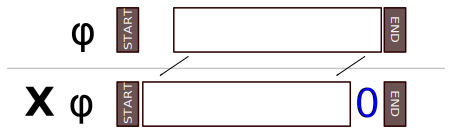
\includegraphics[scale=0.3]{Pattern-X}}~~~
\subfloat[$\mbox{\bf G}\,\varphi$]{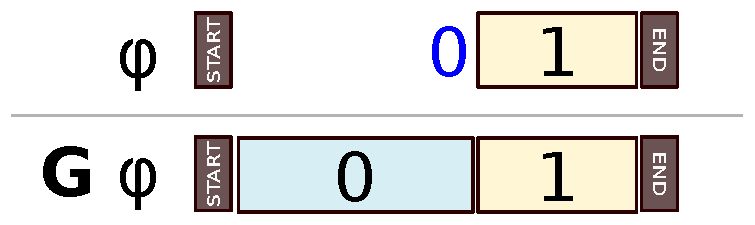
\includegraphics[scale=0.3]{Pattern-G}}~~~
\subfloat[$\varphi\,\mbox{\bf U}\,\psi$]{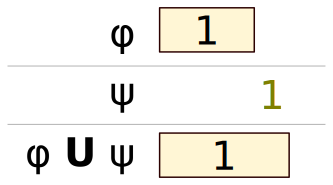
\includegraphics[scale=0.3]{Pattern-U}}
\caption{Une représentation graphique du calcul des trois opérateurs temporels sur bitmaps}
\label{fig:patterns}
\end{figure}

\begin{algorithm}
\caption{Calcul de $\X a$}
\label{alg:next}
\begin{algorithmic}[1]
\Require Bitmap $a$
%\State // X(10101) $\Rightarrow$ (0101)
\State $out \gets$ removeFirstBit($a$)
\State addMany($out$, 0, 1)
\State \Return $out$
\end{algorithmic}
\end{algorithm}

Pour calculer le vecteur de $\G\psi$, il suffit de trouver la plus petite position $i$ de telle sorte que tous les bits suivants sont 1. Dans $B_{\G\psi} $, tous les bits devant $i$ sont mis à 0, et tous les bits d'après (inclusivement) $i$ sont mis à 1. Ainsi, pour mettre en \oe{}uvre cet opérateur avec des bitmaps, nous avons besoin de faire une recherche dans le bitmap $B_{\psi}$ de l'arrière vers l'avant pour trouver la dernière apparition du bit 0, comme on peut le voir de l'Algorithme \ref{alg:global}.

L'opérateur \textbf{F} (montré dans l'Algorithme \ref{alg:future}) est le double de \textbf{G}; son algorithme correspondant fonctionne de la même manière que pour \textbf{G}, en échangeant 0 et 1.

\begin{algorithm}
\caption{Calcul de $\G a$}
\label{alg:global}
\begin{algorithmic}[1]
\Require Bitmap $a$
\State $p \gets$ last(0, $a$)
\If {$p = -1$}
  \State \Return $a$
\Else
  \State $out \gets \langle~\rangle$
  \State addMany($out$, 0, $p + 1$)
  \State addMany($out$, 1, $|a| - p - 1$)
  \State \Return $out$
\EndIf
\end{algorithmic}
\end{algorithm}

\begin{algorithm}
\caption{Calcul de $\F a$}
\label{alg:future}
\begin{algorithmic}[1]
\Require Bitmap $a$
%\State // F(010100) $\Rightarrow$ (111100)
\State $pos \gets$ last(1, $a$)
\If {$pos = -1$}
  \State \Return $a$
\Else
  \State $out \gets$ empty Bitmap
  \State addMany($out$, 1, $pos + 1$)
  \State addMany($out$, 0, $|a| - pos - 1$)
  \State \Return $out$
\EndIf
\end{algorithmic}
\end{algorithm}

D'après la Définition \eqref{eq:until}, s'il y a un indice $j$ avec qui $\overline{s}^j \models \psi$ et $\overline{s}^i$ pour tout $i < j$, alors $\overline{s} \models \varphi\U\psi$. En termes d'opérations bitmap, nous avons besoin de continuer à vérifier s'il y a du bit mis à 1 dans le bitmap $B_{\varphi}$ devant chaque apparition de bit 1 dans $B_{\psi}$ (montré dans l'Algorithme \ref{alg:until}).

\begin{algorithm}
\caption{Calcul de $a \U b$}
\label{alg:until}
\begin{multicols}{2}
\begin{algorithmic}[1]
\Require Bitmaps $a$ et $b$
\State $out \gets \langle~\rangle$
\State $p, a_0, a_1, b_0, b_1 \gets 0$
\While {$p < |a|$}
  \If {$a_1 \leq p$}
    \State $a_1 \gets$ next(1, $a$, $p$)
  \EndIf

  \If {$b_1 \leq p$}
    \State $b_1 \gets$ next(1, $b$, $p$)
  \EndIf

  \If {$a_1 = -1$ or $b_1 = -1$}
    \BreakWhile
  \EndIf

  \State $nearest1 \gets$ min($a_1$, $b_1$)
  \If {$nearest1 > p$}
    %\State // (00..) U (00..) $\Rightarrow$ (00..)
    \State addMany($out$, 0, $nearest1 - p$)
    \State $p \gets nearest1$
    \Continue
  \EndIf

  \If {$p = b_1$}
    %\State // (??..) U (11..) $\Rightarrow$ (11..)
    \If {$b_0 \leq b_1$}
      \State $b_0 \gets$ next(0, $b$, $b_1$)
      \If {$b_0 = -1$}
        \State $b_0 \gets |a|$
      \EndIf
    \EndIf
    \State addMany($out$, 1, $b_0 - p$)
    \State $p \gets b_0$
    \Continue
  \EndIf

  \If {$a_0 \leq a_1$}
    \State $a_0 \gets$ next(0, $a$, $a_1$)
    \If {$a_0 = -1$}
      \State $a_0 \gets |a|$
    \EndIf
  \EndIf
  \If {$a_0 \geq b_1$}
    %\State // (111?..) U (0001..) $\Rightarrow$ (1111..)
    \State addMany($out$, 1, $b_1 - p + 1$)
    \State $p \gets b_1 + 1$
  \Else
    %\State // (11100..) U (00001..) $\Rightarrow$ (00000..)
    \State addMany($out$, 0, $a_0 - p + 1$)
    \State $p \gets a_0 + 1$
  \EndIf
\EndWhile

\If {$b_1 = -1$}
  %\State // (..??) U (..00) $\Rightarrow$ (..00)
  \State addMany($out$, 0, $|a| - |out|$))
\ElsIf {$a_1 = -1$}
  %\State // (..0000) U (..1010) $\Rightarrow$ (..1010)
  \State copyTo($out$, $b$, $p$, $|a| - p$)
\EndIf

\State \Return $out$
\end{algorithmic}
  \end{multicols}
\end{algorithm}

L'opération $\psi \textbf{ W } \varphi$ (la Définition \eqref{eq:wuntil}) est tout à fait semblable à $\psi \textbf{ U } \varphi$, sauf que comme l'implique l'équation \eqref{eq:uw} \citep{huth2004}, l'opération de la première comprend également l'opération $\textbf{G}\psi$. L'Algorithme \ref{alg:wuntil} explique son opération.

\begin{equation} \label{eq:uw}
\psi \textbf{W} \varphi \equiv \psi \textbf{U} \varphi \vee \textbf{G}\psi
\end{equation}

\begin{algorithm}
\caption{Calcul de $a \W b$}
\label{alg:wuntil}
\begin{multicols}{2}
\begin{algorithmic}[1]
\Require Bitmaps $a$ et $b$
\State $out \gets \langle~\rangle$
\State $p, a_0, a_1, b_0, b_1 \gets 0$
\While {p < |a|}
  \If {$a_1 \leq p$}
    \State $a_1 \gets$ next(1, $a$, $p$)
  \EndIf
  \If {$b_1 \leq p$}
    \State $b_1 \gets$ next(1, $b$, $p$)
  \EndIf
  \If {$a_1 = -1$ or $b_1 = -1$}
    \BreakWhile
  \EndIf

  \State $nearest1 \gets$ min($a_1$, $b_1$)
  \If {$nearest1 > p$}
    \State addMany($out$, 0, $nearest1 - p$)
    \State $p \gets nearest1$
    \Continue
  \EndIf

  \If {$p = b_1$}
    \If {$b_0 \leq b_1$}
      \State $b_0 \gets$ next(0, $b$, $b_1$)
      \If {$b_0 = -1$}
        \State $b_0 \gets |a|$
      \EndIf
    \EndIf
    \State addMany($out$, 1, $b_0 - p$)
    \State $p \gets b_0$
    \Continue
  \EndIf

  \If {$a_0 \leq a_1$}
    \State  $a_0 \gets$ next(0, $a$, $a_1$)
    \If {$a_0 = -1$}
      \State $a_0 \gets |a|$
    \EndIf
  \EndIf

  \If {$a_0 \geq b_1$}
    \State addMany($out$, 1, $b_1 - p + 1$)
    \State $p \gets b_1 + 1$
  \Else
    \State addMany($out$, 0, $a_0 - p + 1$)
    \State $p \gets a_0 + 1$
  \EndIf
\EndWhile

\If {$b_1 = -1$}
  \If {$a_1 = -1$}
    \State addMany($out$, 0, $|a| - |out|$)
  \Else
    \State $last0 \gets$ last(0, $a$)
    \If {$last0 = -1$ or $last0 < p$}
      \State addMany($out$, 1, $|a| - |out|$)
    \Else
      \State addMany($out$, 0, $last0 - p + 1$)
      \State addMany($out$, 1, $|a| - |out|$)
    \EndIf
  \EndIf
\ElsIf {$a_1 = -1$}
  \State copyTo($out$, $b$, $|b| - b_1 - 1$, $|b| - b_1$)
\EndIf

\State \Return $out$
\end{algorithmic}
\end{multicols}
\end{algorithm}

Comme le double de l'opérateur \textbf{U}, l'opérateur \textbf{R} défini dans \eqref{eq:release} a besoin de faire une union de deux parties pour la formule $\psi \textbf{ R } \varphi$: la première partie vise à détecter si existent $i, j (0 \leq i < j) $ qui rendent la séquence $\pi^i, \pi^{i + 1}, ... \pi^j $ satisfaite à $\varphi$ lorsque $\pi^j$ satisfait $\psi$; et la seconde est tout simplement $G\varphi$. L'Algorithme \ref{alg:release} décrit cette procédure.

\begin{algorithm}
\caption{Calcul de $a \R b$}
\label{alg:release}
\begin{multicols}{2}
\begin{algorithmic}[1]
\Require Bitmaps $a$ et $b$
\State $out \gets \langle~\rangle$
\State $p, a_0, a_1, b_0, b_1 \gets 0$
\While {$p < |a|$}
  \If {$b_1 \leq p$}
    \State $b_1 \gets$ next(1, $b$, $p$)
  \EndIf
  \If {$b_1 = -1$}
    \BreakWhile
  \EndIf

  \If {$b_1 > p$}
    \State addMany($out$, 0, $b_1 - p$)
    \State $p \gets b_1$
    \Continue
  \EndIf

  \If {$a_1 \leq p$}
    \State $a_1 \gets$ next(1, $a$, $p$)
  \EndIf
  \If {$a_1 = -1$}
    \BreakWhile
  \EndIf

  \If {$b_0 \leq b_1$}
    \State $b_0 \gets$ next(0, $b$, $b_1$)
    \If {$b_0 = -1$}
      \State $b_0 \gets |a|$
    \EndIf
  \EndIf
  \If {$a_1 \geq b_0$}
    \State addMany($out$, 0, $b_0 - p + 1$)
    \State $p \gets b_0 + 1$
    \Continue
  \EndIf

  \If {$a_0 \leq a_1$}
    \State $a_0 \gets$ next(0, $b$, $a_1$)
    \If {$a_0 = -1$}
      \State $a_0 \gets |a|$
    \EndIf
  \EndIf
  \State $nearest0 \gets$ min($a_0$, $b_0$)
  \State addMany($out$, 1, $nearest0 - p$)
  \State $p \gets nearest0$
\EndWhile

\If {$a_1 = -1$ and $b_1 \neq -1$}
  \State $last0 \gets$ last(0, $b$)
  \If {$last0 = -1$ and $last0 < p$}
    \State addMany($out$, 1, $|a| - |out|$)
  \Else
    \State addMany($out$, 0, $last0 - p + 1$)
    \State addMany($out$, 1, $|a| - |out$)
  \EndIf
\Else
  \State addMany($out$, 0, $|a| - |out|$)
\EndIf

\State \Return $out$
\end{algorithmic}
\end{multicols}
\end{algorithm}

\subsection{Discussion}

Un point intéressant des derniers trois algorithmes est que les bitmaps $a$ et $b$ ne sont pas toujours traversés de façon linéaire. Au contraire, des blocs entiers de chaque bitmap peuvent être contournés pour atteindre directement le prochain bit de 0 ou 1, selon le cas. Il faut remarquer que ceci est possible uniquement si la trace est complètement connue à l'avance avant de commencer à évaluer une formule (et de plus, la trace est traversée vers l'arrière). Par conséquent, la solution proposée est un exemple d'un moniteur en mode hors ligne qui n'est pas simplement un moniteur en ligne qui est nourri d'événements d'une trace pré-enregistrée un par un: il exploite la possibilité d'un \emph{accès aléatoire} à des parties de la trace qui est seulement possible dans un réglage hors ligne.

Cet exemple montre l'un des avantages de notre technique proposée en termes de complexité. En effet, la lecture du journal d'origine pour la création des bitmaps fragmentés peut être faite en temps linéaire (et en une seule passe pour tous les symboles propositionnels à la fois). Cependant, une fois que ces bitmaps initiaux sont calculés, un grand nombre d'opérations nécessaires ne requièrent plus un traitement linéaire de la trace. Par exemple, l'évaluation $\X\varphi$ nécessite un simple décalage de bits, qui peut être fait dans une seule opération de CPU pour 64 bits à la fois, et potentiellement beaucoup plus si la compression est appliquée.\footnote{Le décalage à gauche de bits d'un bloc compressé est le bloc lui-même, aussi longtemps que le premier bit du prochain bloc à droite a la même valeur.} De la même façon, la recherche du prochain bit de 0 ou 1 requiert rarement la recherche linéaire, car l'utilisation de la compression permet de contourner des mots pleins avec une opération. Le calcul du bitmap pour un opérateur \textbf{F} ou \textbf{G} exige une seule recherche semblable pour toute la trace.

Un autre point intéressant est le fait que les opérateurs \textbf{F} et \textbf{G} sont monotones. Comme on peut le voir dans la Figure \ref{fig:patterns}, le bitmap qui est résulte est sous forme de $0^*1^*$ (ou l'inverse). Ainsi, un bitmap très simple se propage vers d'autres algorithmes; il peut être fortement compressé, et rend toute recherche du prochain 0 ou 1 trivial. Bien que les bitmaps résultant des applications de \textbf{U}, de \textbf{W} et de \textbf{R} ne produisent pas de tels vecteurs simples, ils ont toujours une structure relativement régulière qui est aussi souple pour une compression raisonnable.

%% }}} --- Subsection

%% }}} --- Section

%% ------------------
%% Section: expériences
%% ------------------
\section{Implémentation et expériences}\label{sec:bm:experiments} %% {{{

Alors que la complexité du pire cas de chaque algorithme présenté dans la section précédente est encore $O(n)$ (où $n$ est la taille du bitmap d'entrée), nous soupçonnons que la performance pratique devrait être nettement meilleure. Par conséquent, dans cette section, nous décrivons des expériences en vue d'atteindre les objectifs suivants:

\begin{enumerate}
\item Tester la performance des algorithmes LTL fondamentaux;
\item Tester la performance de l'application récursive de ces algorithmes sur des formules LTL complexes;
\item Évaluer la performance et l'espace économique encourus par l'utilisation de la compression.
\end{enumerate}

\subsection{Préparation des expériences} %% {{{

Comme un moyen d'éviter les coûts d'entrées ou de sorties de disques à l'exécution, nous chargeons tous les fichiers pertinents dans la mémoire avant les calculs. Ainsi, bien que l'utilisation de bitmaps puisse considérablement réduire l'exigence de mémoire, nous avons préparé un poste de travail qui a un processeur d'Intel Xeon E5-2630 v3 et 48 Go de mémoire.

Tous les codes sont mis en \oe{}vre en Java qui prend en soi la responsabilité de la gestion de la mémoire et de la collecte des ordures. En ce qui concerne le délai causé par la collecte des ordures (GC) et surtout Full-GC, nous avons manuellement effectué \textit{System.gc()} avant et après chaque calcul de formules pour fournir un environnement d'exécution qui était aussi ``propre'' que possible.

Le Tableau \ref{table:bmlibs} montre les librairies utilisées pour différents types de bitmap. Afin de mettre en \oe{}uvre toutes les opérations LTL, nous avons modifié les codes des librairies pour ajouter les fonctions nécessaires énumérées dans le Tableau \ref{tbl:bm:bmhelpers} et optimiser les fonctions de sorte que les complexités en temps des opérateurs deviennent $O(m)$ où $m$ est le nombre de séquences de bits consécutifs de 0 ou de 1.

\begin{table}
\centering
\begin{tabular}{|c|l|}
\hline
Librairie bitmap & Source \\
\hline
Non compressée & \texttt{java.util.BitSet} à partir de SDK Java  \\
\hline
\multirow{2}{*}{WAH} & Originale:\ \ \url{https://github.com/metamx/extendedset} \\
& Modifiée: \url{https://github.com/phoenixxie/extendedset} \\
\hline
\multirow{2}{*}{Concise} & Originale:\ \ \url{https://github.com/metamx/extendedset} \\
& Modifiée: \url{https://github.com/phoenixxie/extendedset} \\
\hline
\multirow{2}{*}{EWAH} & Originale:\ \ \url{https://github.com/lemire/javaewah} \\
& Modifiée: \url{https://github.com/phoenixxie/javaewah} \\
\hline
Roaring & \url{https://github.com/lemire/RoaringBitmap} \\
\hline
\end{tabular}
\caption{Librairies bitmap}
\label{table:bmlibs}
\end{table}

En raison du manque de soutien de l'accès aléatoire pour les algorithmes de modèles RLE de compression bitmap, nous ne pouvons pas énumérer les bits de la même manière qu'un bitmap non compressé. Par conséquent, nous avons conçu une structure de données \emph{itérateur} pour stocker non seulement l'indice absolu du bit actuel dans le correspondant bitmap non compressé, mais aussi l'indice relatif dans le bitmap compressé. Prenant l'exemple de la fonction \textbf{next(1, x)}, si l'indice relatif actuel est dans un mot de séquence de 0, la recherche dans ce mot est inutile, et nous passons simplement au mot suivant; si l'indice est dans un mot de séquence de 1, on retourne l'index actuel; cependant, si l'indice est dans un mot littéral, nous devons chercher le bit 1 dans le mot de $ulen$ bits.

Pour les expériences, nous avons développé un générateur de données aléatoires. Chaque fois qu'il génère $5 \times 10^7$ tuples, et chaque tuple contient trois nombres aléatoires ($a, b, c$) liés à trois inégalités simples: $a > 0$, $b > 0$ et $c \leq 0$, qui seront étiquetées comme $s_0$, $s_1$ et $s_2$, respectivement. Selon \eqref{eq:ap}, les valeurs vrai/faux de ces trois déclarations sont composées de propositions atomiques. Quand un tuple a été passé aux trois déclarations, nous avons obtenu trois valeurs booléennes dont chacune a ensuite été transformée en bit de 1 ou de 0 dans le bitmap correspondant à l'un des trois états. Lorsque tous les tuples ont été traités, nous avions trois bitmaps ayant 50 millions de bits chacun.

\subsection{Opérateurs LTL fondamentaux} %% {{{

Une première expérience est formée de l'évaluation de la performance, en termes de temps de calcul, pour évaluer un vecteur de bits sur chaque opérateur propositionnel et temporel.

Dans la première expérience, nous avons effectué 100 passes d'un benchmark sur les opérateurs fondamentaux avec des bitmaps non compressés. Dans chaque passe, les données d'expérience ont été régénérées et transmises aux déclarations relationnelles à partir desquelles les bitmaps ont été créés. Puis les formules ont été exécutées avec les bitmaps. Dans la dernière étape, nous avons calculé le temps moyen d'exécution d'une passe pour chaque opérateur LTL, et le nombre de bits traités par seconde.

Le Tableau \ref{tbl:bm:basicops} montre que les opérateurs de logiques propositionnelles étaient plus rapides que la plupart des opérateurs de logiques temporelles. Parmi les opérateurs de logiques temporelles, les opérateurs binaires sont plus lents que ceux unaires parce que les premiers requièrent plus d'opérations que les seconds, particulièrement dans la situation où plusieurs séquences de 0s et de 1s sont mélangées dans le bitmap. Les opérateurs duals \textbf{G} et \textbf{F} ont des algorithmes similaires, mais \textbf{F} a pris étonnamment trois fois plus de temps que \textbf {G}. Ceci peut être expliqué par le fait que pour un bitmap d'entrée assez randomisé, \textbf{F} ajoute plus de bits de 1s que de 0s à son bitmap de sortie, tandis que \textbf{G} ajoute plus de bits de 0s que de 1s. Bien que l'implémentation de \texttt{BitSet} en Java puisse mettre un bit à 1 et à 0\footnote{\url{https://docs.oracle.com/javase/8/docs/api/java/util/BitSet.html}}, elle ne fait actuellement rien quand elle est demandée de mettre à 0 un nouveau bit dont l'indice est au-delà de sa taille, c'est-à-dire l'ajout d'un bit 0. Il en résulte un traitement asymétrique de bits de 0s et de 1s dans le bitmap.

\begin{table}
\centering
\small
\begin{tabular}{|c|c|c|c|c|}
\hline
Formule & Temps\ Min. & Temps\ Max. & Temps\ Moyen & Débit \\
& (ms) & (ms) & (ms) & (b/s) \\
\hline
$\neg s_0$ & 0 & 15 & 6.18 & $8.09 \times 10^{9}$ \\
\hline
$s_0 \wedge s_1$ & 0 & 16 & 5.86 & $8.53 \times 10^{9}$ \\
\hline
$s_0 \vee s_1$ & 0 & 16 & 5.8 & $8.62 \times 10^{9}$ \\
\hline
$s_0 \rightarrow s_1$ & 0 & 16 & 4.66 & $1.07 \times 10^{10}$ \\
\hline
$\X s_0$ & 0 & 16 & 8.93 & $5.60 \times 10^{9}$ \\
\hline
$\G s_0$ & 46 & 63 & 51.3 & $9.75 \times 10^8$ \\
\hline
$\F s_0$ & 140 & 174 & 150.55 & $3.32 \times 10^8$ \\
\hline
$s_0 \U s_1$ & 1562 & 2017 & 1747.05 & $5.72 \times 10^7$ \\
\hline
$s_0 \W s_1$ & 1531 & 1957 & 1685.71 & $5.93 \times 10^7$ \\
\hline
$s_0 \R s_1$ & 1735 & 2188 & 1961.37 & $5.10 \times 10^7$ \\
\hline
\end{tabular}
\vskip 8pt
\caption{Temps d'exécution d'évaluation de chaque opérateur LTL sur un vecteur de bits, sans l'utilisation de librairie de compression.}
\label{tbl:bm:basicops}
\end{table}

%% }}} --- Subsection

\subsection{Formules complexes} %% {{{

Les résultats de cette première expérience suggèrent que les opérateurs de logiques propositionnelles, les opérateurs de logiques temporelles unaires et les opérateurs de logiques temporelles binaires ont des magnitudes différentes de vitesse de traitement; par conséquent, nous pouvons diviser les opérateurs en trois groupes.

Au début de cette deuxième expérience, nous avons composé diverses combinaisons d'opérateurs en 14 formules LTL avec l'aide de l'outil \emph {randltl} de la librairie \textit{Spot}\footnote{\url{https://spot.lrde.epita.fr/index.html}}; les formules sont présentées dans le Tableau \ref{tbl:bm:complex-formulas}. Ensuite, nous avons également effectué un benchmark de 50 passes sur ces formules avec des bitmaps non compressés. Dans chaque cycle les données ont été régénérées et ré-exécutées avec les 14 formules. Nous avons mesuré le temps d'exécution de chaque cycle et calculé le coût moyen en temps et la vitesse de traitement comme avant.

\begin{table}[h]
\begin{footnotesize}

\begin{equation}\tag{F1}
\G ((s_2 \mathrel{\rightarrow} \F (\mathop{\neg}(s_1 \U  s_2) \W  (s_2 \mathrel{\vee} \G s_1))) \W  (\mathop{\neg}\F (s_0 \R  \X s_2) \W  ((s_0 \mathrel{\wedge} s_2 \mathrel{\wedge} \F s_2) \U  s_0)))
\end{equation}
%
\squeeze
%
\begin{equation}\tag{F2}
\F (\mathop{\neg}(s_2 \mathrel{\rightarrow} \X (s_0 \U  s_1)) \U  (\mathop{\neg}(s_0 \mathrel{\vee} \F \X (s_0 \U  (\X (\F s_1 \W  s_1) \R  s_1))) 
\U  (s_0 \R  \G s_2)))
\end{equation}
%
\squeeze
%
\begin{equation}\tag{F3}
\X \F ((s_1 \mathrel{\vee} s_2 \mathrel{\vee} (\G (s_0 \mathrel{\vee} s_1 \mathrel{\vee} \mathop{\neg}s_1) \mathrel{\wedge} \X \mathop{\neg}s_0)) \mathrel{\rightarrow} \\
((\mathop{\neg}s_0 \mathrel{\rightarrow} (s_0 \mathrel{\wedge} \mathop{\neg}s_1)) \mathrel{\wedge} \G s_0))
\end{equation}
%
\squeeze
%
\begin{equation}\tag{F4}
\X (\mathop{\neg}\G (s_0 \mathrel{\rightarrow} s_2) \mathrel{\rightarrow} \F (s_1 \mathrel{\wedge} ((\F (s_0 \mathrel{\wedge} s_2) \mathrel{\rightarrow} s_1) \mathrel{\rightarrow} \X \mathop{\neg}s_2) \mathrel{\wedge} \G (s_2 \mathrel{\rightarrow} (s_2 \mathrel{\wedge} \F s_1))))
\end{equation}
%
\squeezemore
%
\begin{multline}\tag{F5}
\mathop{\neg}((s_0 \U  (\mathop{\neg}(\mathop{\neg}s_0 \mathrel{\wedge} s_2) \mathrel{\vee} (\mathop{\neg}s_0 \W  (s_2 \mathrel{\rightarrow} s_0)))) \\
\W  \mathop{\neg}s_0) \mathrel{\vee}
(s_1 \R  ((s_1 \mathrel{\vee} (s_0 \W  s_2)) \W  (\mathop{\neg}s_0 \W  s_2)))
\end{multline}
%
\squeeze
%
\begin{equation}\tag{F6}
(s_1 \W  ((s_2 \mathrel{\rightarrow} (\mathop{\neg}s_2 \R  \mathop{\neg}(\mathop{\neg}s_1 \W  s_0))) \W  (\mathop{\neg}s_1 \mathrel{\vee} \mathop{\neg}((\mathop{\neg}s_2 \mathrel{\rightarrow} s_1) \mathrel{\rightarrow} \mathop{\neg}s_0)))) \W  (s_0 \R  \mathop{\neg}s_2)
\end{equation}
%
\squeezemore
%
\begin{multline}\tag{F7}
\X (((\F s_2 \R  s_0) \U  \F s_0) \R  \G ((s_2 \W  s_1) \W  \\
(((\G s_2 \U  s_1) \R  \X s_0) \R  (s_2 \W  ((s_2 \R  \X s_2) \W  s_1)))))
\end{multline}
%
\squeezemore
%
\begin{equation}\tag{F8}
(\G (s_0 \R  \F s_1) \U  \F s_2) \W  \G ((s_1 \U  s_2) \R  ((\G \X s_0 \U  (s_2 \W  s_0)) \W  \F ((\G s_1 \U  s_2) \R  s_2)))
\end{equation}
%
\squeeze
%
\begin{equation}\tag{F9}
\G \F (\G \F s_0 \mathrel{\wedge} \F \X \G s_1 \mathrel{\wedge} \G \F \X \X \X \G \X \F \G s_2)
\end{equation}
%
\squeeze
%
\begin{equation}\tag{F10}
\F \G \F \X (\X s_2 \mathrel{\wedge} \X \G \X \X \G \F (\G \X \F s_1 \mathrel{\wedge} \X \G s_0))
\end{equation}
%
\squeeze
%
\begin{equation}\tag{F11}
\mathop{\neg}(((s_0 \mathrel{\vee} s_2) \mathrel{\rightarrow} (\mathop{\neg}(s_2 \mathrel{\wedge} (\mathop{\neg}s_2 \mathrel{\rightarrow} \mathop{\neg}(s_0 \mathrel{\wedge} (s_0 \mathrel{\vee} \mathop{\neg}s_1)))) \mathrel{\vee} (s_0 \mathrel{\wedge} \mathop{\neg}s_0))) \mathrel{\vee} (\mathop{\neg}s_0 \mathrel{\wedge} (s_0 \mathrel{\vee} s_2)))
\end{equation}
%
\squeezemore
%
\begin{multline}\tag{F12}
(s_1 \mathrel{\wedge} \mathop{\neg}s_2 \mathrel{\wedge} (s_2 \mathrel{\rightarrow} s_0)) \mathrel{\vee} \mathop{\neg}((s_0 \mathrel{\wedge} \mathop{\neg}s_0) \mathrel{\rightarrow} s_1) \mathrel{\vee} \\
((s_2 \mathrel{\vee} (s_1 \mathrel{\rightarrow} s_0)) \mathrel{\wedge} ((s_0 \mathrel{\wedge} \mathop{\neg}s_2 \mathrel{\wedge} (s_1 \mathrel{\rightarrow} s_0)) \mathrel{\rightarrow} s_0))
\end{multline}
%
\squeezemore
%
\begin{multline}\tag{F13}
(((s_0 \W  s_2) \W  s_0) \U  ((s_1 \U  (((s_1 \W  s_2) \W  (s_1 \R  (s_1 \R  s_0))) \W  s_2)) \W  s_2)) \W  \\
((s_0 \R  s_1) \R  (((s_2 \U  s_1) \U  s_1) \R  ((s_0 \W  s_2) \W  s_1)))
\end{multline}
%
\squeezemore
%
\begin{multline}\tag{F14}
((((s_1 \U  s_2) \U  (s_2 \U  s_1)) \U  s_1) \R  (s_1 \R  s_2)) \U  (((s_2 \W  ((s_0 \W  \\
((s_2 \R  s_0) \R  s_1)) \U  s_1)) \W  s_0) \W  (((s_0 \R  s_1) \R  (s_0 \W  s_1)) \U  s_0))
\end{multline}

\end{footnotesize}
\vskip 8pt
\caption{Les formules LTL complexes évaluées expérimentalement}
\label{tbl:bm:complex-formulas}
\end{table}

Comme il est indiqué dans le Tableau \ref{tbl:bm:complex}, trois groupes d'opérateurs ont différentes échelles de vitesse de traitement. Les combinaisons ayant des opérateurs de logiques temporelles et binaires ont toujours pris plus de temps que d'autres, et les formules F13 et F14 sont les plus lentes. Ce résultat montre également que notre solution peut manipuler un assez grand nombre de bits (événements de la trace) par seconde, allant de millions à milliards.

\begin{table}[h]
\centering
\small
\begin{tabular}{|c|c|c|c|c|c|c|c|}
\hline
Formule & Opérateurs & Opérateurs & Opérateurs & Temps & Temps & Temps & Bits/second \\
No. & Logiques & Temporels & Temporels. & Min.  & Max. & Avg. & Approx. \\
 & Props. & Unaires & Binaires & (ms) & (ms) & (ms) &  \\
\hline
F1 & 6 & 6 & 6 & 10454 & 14205 & 11483.02 & $1.31 \times 10^7$ \\
\hline
F2 & 4 & 7 & 7 & 7728 & 10673 & 8937.59 & $1.68 \times 10^7$  \\
\hline
F3 & 13 & 5 & 0 & 281 & 422 & 326.63 & $4.59 \times 10^8$  \\
\hline
F4 & 11 & 7 & 0 & 422 & 704 & 560.58 & $2.68 \times 10^8$  \\
\hline
F5 & 11 & 0 & 7 & 8532 & 10496 & 9374.5 & $1.60 \times 10^7$  \\
\hline
F6 & 12 & 0 & 6 & 7280 & 9357 & 7934.6 & $1.89 \times 10^7$  \\
\hline
F7 & 0 & 7 & 11 & 12330 & 15004 & 13413.91 & $1.18 \times 10^7$  \\
\hline
F8 & 0 & 8 & 10 & 9442 & 11833 & 10428.37 & $1.44 \times 10^7$  \\
\hline
F9 & 2 & 16 & 0 & 431 & 1155 & 682.68 & $2.20 \times 10^8$  \\
\hline
F10 & 2 & 16 & 0 & 375 & 857 & 472.76 & $3.17 \times 10^8$  \\
\hline
F11 & 18 & 0 & 0 & 31 & 56 & 45.18 & $3.32 \times 10^9$  \\
\hline
F12 & 18 & 0 & 0 & 46 & 68 & 51.58 & $2.91 \times 10^9$  \\
\hline
F13 & 0 & 0 & 18 & 22768 & 27308 & 24825.21 & $6.04 \times 10^6$  \\
\hline
F14 & 0 & 0 & 18 & 22800 & 27481 & 24877.67 & $6.03 \times 10^6$  \\
\hline
\end{tabular}
\vskip 8pt
\caption{Temps d'exécution de l'évaluation des formules LTL du Tableau \ref{tbl:bm:complex-formulas}, sans l'utilisation de librairie de compression.}
\label{tbl:bm:complex}
\end{table}

%% }}} --- Subsection

\subsection{Utilisation de compression bitmap} %% {{{

Selon les algorithmes de modèles RLE, le taux de compression dépend principalement de la longueur de bits consécutifs de 0s ou de 1s. De ce fait, dans cette expérience, nous avons modifié le générateur pour lui permettre de répéter le même tuple un certain nombre de fois: 1, 32 et 64. Ce nouveau mécanisme est en mesure d'assurer l'existence de séquences continues d'une longueur minimum ($slen$) dans les bitmaps générés. Intuitivement, lorsque la valeur de $slen$ augmente, le nombre de séquences diminue; par conséquent, les algorithmes de modèles RLE devraient avoir de meilleures performances qu'un bitmap non compressé.

\begin{figure}[h]
\begin{center}
\centering
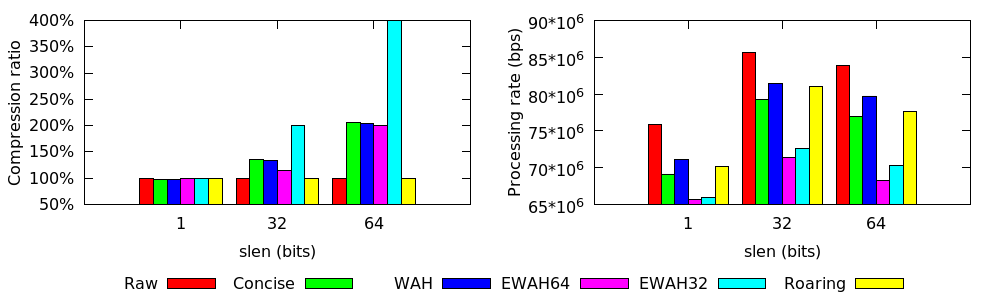
\includegraphics[width=\linewidth]{states.png}
\caption{Génération de bitmaps avec les algorithmes de compression}
\label{img:states}
\end{center}
\end{figure}

Dans la première partie de l'expérience, nous avons généré les bitmaps avec différents algorithmes et les différentes valeurs de $slen$, puis calculé les taux de compression. Le résultat dans la Figure \ref{img:states} confirme l'hypothèse selon laquelle quand $slen < wlen$ (où $wlen$ est la longueur d'un mot), le bitmap ne peut pas être bien compressé par un algorithme de modèle RLE, et dans ce cas, l'algorithme EWAH se comporte un peu mieux que les autres en raison de son coût structurel plus petit. Lorsque $slen$ augmente à 32 et à 64, c.-à-d. $slen \geq wlen$, les algorithmes RLE commencent à bien fonctionner et le taux de compression lors de $slen = 64$ est évidemment meilleur que celui lors de $slen = 32$. Dans la Figure \ref{img:states}, nous pouvons également voir que quand $slen$ est égal à 1, à 32 et à 64, EWAHs sont plus lents que WAH, Concise et Roaring.

Dans la deuxième partie de l'expérience, nous avons mesuré les performances des bitmaps compressés lors de l'application des algorithmes pour tous les opérateurs fondamentaux et tous les formules LTL dans les expériences précédentes. Les résultats détaillés couvrant tous les opérateurs et les formules peuvent être trouvés dans l'Annexe \ref{appendixa}.

À cette fin, nous avons choisi les formules F1 et F14 de l'expérience précédente, car F1 contient tous les opérateurs et les conjonctions de LTL et F14 est la plus lente de toutes les formules dans l'expérience précédente. Nous avons à nouveau effectué le benchmark 100 fois; dans chaque cycle, la formule a été évaluée par un groupe de bitmaps d'entrée de la dernière étape et nous avons enregistré le coût de temps de chaque algorithme bitmap et de chaque longueur de bits consécutifs.

\begin{figure}[h]
\begin{center}
\centering
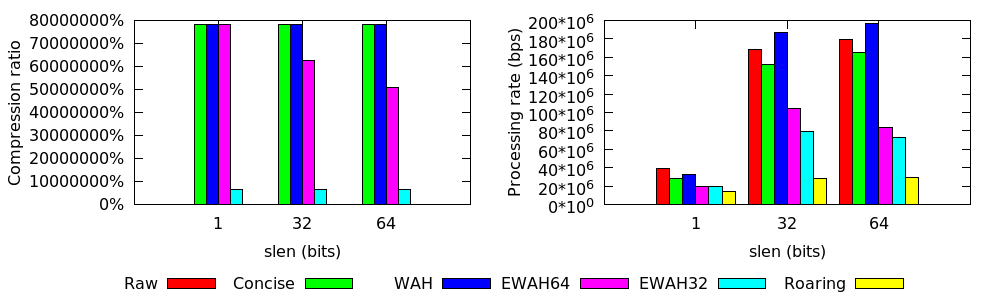
\includegraphics[width=\linewidth]{p11.png}
\caption{Comparaison du taux de compression et de la vitesse de traitement de la formule F1, avec diverses librairies de compression bitmap et différentes valeurs de $slen$}
\label{img:f1}
\end{center}
\end{figure}

\begin{figure}[h]
\begin{center}
\centering
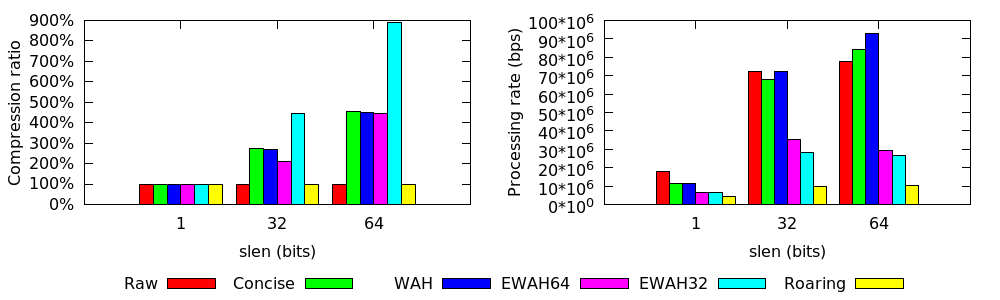
\includegraphics[width=\linewidth]{p24.png}
\caption{Comparaison du taux de compression et de la vitesse de traitement de la formule F14, avec diverses librairies de compression bitmap et différentes valeurs de $slen$}
\label{img:f14}
\end{center}
\end{figure}

Selon les Figures \ref{img:f1} et \ref{img:f14}, la performance des algorithmes de modèles RLE, WAH, EWAH et Concise est évidemment liée à la valeur de $slen$. La Figure \ref{img:f1} suggère également que la présence des opérateurs \textbf{G} et \textbf{F} peut grandement augmenter la longueur de bits consécutifs de même valeur, qui à leur tour peuvent être bien compressés par des algorithmes de modèles RLE. Dans un tel cas, plusieurs algorithmes ont de meilleures performances que le bitmap non compressé lors de l'augmentation de $slen$.

%% }}} --- Subsection

%% }}} --- Section

%% ------------------
%% Section: related work
%% ------------------
\section{Travaux connexes}\label{sec:bm:related} %% {{{

La perspective de l'utilisation de propriétés physiques de matériel pour améliorer les performances de la vérification de l'exécution a déjà été étudiée depuis peu. Par exemple, Pellizzoni \etal\@ \citep{pellizzoni2008hardware} ont utilisé du matériel dédié commercial-off-the-shelf (COTS) \citep{emerson1990temporal} pour faciliter le monitoring de l'exécution de systèmes embarqués critiques dont les propriétés ont été exprimées en logique temporelle linéaire en temps passé (ptLTL).

Comme le nombre de c\oe{}urs (GPU ou CPU multi-c\oe{}urs) dans le matériel de base ne cesse de croître, la recherche de l'exploitation des processeurs disponibles ou des c\oe{}ur disponibles pour paralléliser les tâches et les calculs apporte un défi et aussi une occasion d'améliorer l'architecture de la vérification de l'exécution. Par exemple, Ha \etal\@ \citep{ha2009concurrent} ont présenté une conception de tamponnage de \emph{Cache-friendly Asymmetric Buffering (CAB)} pour améliorer les communications entre l'application et le moniteur d'exécution en utilisant le cache partagé de l'architecture multi-c\oe{}urs; Berkovich \etal\@ \citep{DBLP:journals/fmsd/BerkovichBF15} a proposé une solution à base de GPU qui utilise efficacement les c\oe{}urs disponibles du GPU, de sorte que le moniteur conçu et implémenté avec leur méthode puisse fonctionner en parallèle avec le programme cible et évaluer des propriétés LTL.

Le travail antérieur de l'un des auteurs \citep{jocasa} introduit un algorithme pour la vérification automatisée de formules de logiques temporelles linéaires sur des traces d'événements, en utilisant un cadre de cloud computing appelé MapReduce de plus en plus populaire. L'algorithme peut traiter plusieurs fragments arbitraires de la trace en parallèle, et calculer le résultat final à travers un cycle d'exécution d'instances de MapReduce.
La technique proposée manipule des objets appelés \emph{tuples}, qui sont de la forme $\langle \phi, (n, i)\rangle$, et sont interprétés comme la déclaration ``the process is at iteration $i$, and LTL formula $\phi$ is true for the suffix of the current trace starting at its $n$-th event''. On peut voir que cette déclaration correspond exactement au fait, dans la présente solution, que la $n$-ème position du bitmap généré par l'évaluation de $\phi$ contient la valeur 1.

Outre cette similitude, toutefois, les deux techniques sont radicalement différentes. Puisque la méthode de MapReduce fonctionne sur les tuples un par un, alors que la présente solution manipule les bitmaps entiers, les algorithmes pour chaque opérateur LTL ont peu en commun (en particulier celui de \textbf{U}). Lorsque la méthode de MapReduce obtient sa vitesse du traitement de plusieurs sous-formules sur des machines différentes, notre solution présente est efficace parce que certaines opérations (comme conjonction) peuvent être calculées simultanément pour de nombreux événements adjacents dans un seul cycle de CPU. En plus, un inconvénient de la solution MapReduce est le grand nombre de tuples générés, et l'impossibilité de compression du volume de données.

Comme on peut le voir, il y a eu plusieurs tentatives de parallélisme appuyant et de propriétés de matériel pour évaluer des expressions temporelles sur des traces. Cependant, pour autant que l'on le sache, notre travail est le premier à obtenir l'amélioration de performance au niveau des \emph{structures de données} pour évaluer ces expressions.

%% }}} --- Section

%% ------------------
%% Section: conclusion
%% ------------------
\section{Conclusion et perspectives}\label{sec:bm:conclusion} %% {{{

Nous avons proposé une solution pour l'évaluation hors ligne de formules LTL au moyen de manipulations de bitmaps. Dans un tel contexte, les prédicats propositionnel sur des événements individuels d'états d'une trace sont mappés aux bits d'un vecteur (``bitmap'') qui sont ensuite manipulés pour mettre en \oe{}uvre chaque opérateur LTL. En plus du fait que les manipulations de bitmaps sont en soi très efficaces, nos algorithmes profitent du fait que la trace est complètement connue à l'avance, et que l'accès aléatoire à une position quelconque de cette trace permet de contourner de grands blocs d'événements pour accélérer l'évaluation.

Pour cette raison, notre solution est un important exemple d'un algorithme d'évaluation hors ligne qui exploite le fait que cela fonctionne bien en mode hors ligne --- il n'est pas un algorithme en ligne qui lit les événements à partir d'une trace pré-enregistrée un par un. En fait, dans certains cas (comme l'opérateur \textbf{U}), la trace est même évaluée à partir de la fin, plutôt qu'à partir du début. Un approfondi benchmark de performance pour les opérateurs fondamentaux et les formules LTL complexes a prouvé la faisabilité de la solution, et a montré comment les événements d'une trace peuvent être traités à une vitesse allant de millions à milliards d'événements par seconde.

Pour exploiter davantage le potentiel de bitmaps, nous avons présenté des algorithmes de compression bitmap dans notre solution et les avons intégrés dans notre benchmark. Dans les expériences, comme nous l'espérions, notre solution a démontré sa capacité de compresser facilement les bitmaps creux et d'accélérer les opérations LTL quand il y a un certain nombre de bits consécutifs avec la même valeur. Nous avons expliqué, comment de nombreux opérateurs LTL augmentent naturellement la régularité des bitmaps qu'ils traitent.

De toute évidence, cette solution ne convient qu'à l'évaluation hors ligne. Cependant, les résultats prometteurs obtenus dans notre implémentation conduisent à un grand nombre d'extensions et d'améliorations potentielles basées sur la méthode actuelle. Tout d'abord, l'algorithme peut être réutilisé comme base pour d'autres langages temporels qui se croisent avec LTL, tels que PSL \citep{IntroPSLBook}. D'autre part, cette technique pourrait être étendue pour prendre en considération des paramètres et une quantification de données. Enfin, on pourrait aussi envisager la parallélisation de l'évaluation des grands segments de bitmaps sur plusieurs machines.
%% }}} --- Section

%% :folding=explicit:wrap=soft:mode=latex:
